\section{Verwendete Technologien}

Es werden folgende Technologien verwendet:

\begin{itemize}
    \item Raspberry Pi Zero W: Weil er klein und kostengünstig ist
    \item Node.JS: für den Webserver (Livestream), GPIO Zugriff (Bewegungssensor), Bilder, Mail
\end{itemize}

Verwendete Node.JS libraries:

\begin{itemize}
    \item express: Für den Webserver/Livestream
    \item hls.js: Livestream in HLS format
    \item ip: IP-Addresse auslesen
    \item nodemailer: Mail mit IP/Bild senden
    \item onoff: Für GPIO pins
    \item pi-camera: Um auf die Kamera zuzugreifen
\end{itemize}

Um den Schaltplan zu verfassen wird die Desktop-Applikation \textbf{Fritzing} verwendet.

\clearpage
\section{Research}

\subsection{Raspberry Setup}

Die initiale Konfiguration des Raspberry Pi's erfolgt mittels der \texttt{raspi-info.md} Dokumentation.

\subsection{Abtastrate der Informationen}

Da eine fixe Abtastrate ineffizient wäre, wird ein GPIO callback verwendet um ein Bild zu senden.

Der Bewegungssensor wird folgendermaßen initialisiert:

\begin{listing}
    \begin{code}{js}
    const pir = new Gpio(17, 'in', 'both')
    \end{code}
    \caption{GPIO Erstellung in JavaScript}
\end{listing}

Mittels dem erstellten \texttt{Gpio} Objekt kann ein Callback registriert werden:

\begin{listing}
    \begin{code}[firstnumber=last]{js}
    pir.watch(function(err, value) {
        // Bewegungsmelder callback
        if (err) exit()
        console.log('Intruder detected')
        if (value == 1) {
            mail.sendMail()
        }
    })
    \end{code}
    \caption{GPIO Callback registrierung mittels watch in JavaScript}
\end{listing}

Zusätzlich wird ein Livestream über die Website erstellt, wobei keine fixe Abtastrate verwendet wird.

\clearpage
\subsection{Aggregierung der Daten}
Bei jeder Rising Edge des Bewegungssensors wird eine Mail an den Besitzer gesendet. Der Code schaut folgendermaßen aus:
\begin{listing}
    \begin{code}[firstnumber=last]{js}
    const pir = new Gpio(17, 'in', 'both')
    pir.watch(function(err, value) {
        if (err) exit()

        console.log('Intruder detected')

        if (value == 1) {
            mail.sendMail()
        }
    })
    \end{code}
    \caption{Sender der Mail bei Erkennung einer Bewegung bzw. Rising Edge des Sensors}
\end{listing}

\subsection{Schnittstellendefinition}
Der Bewegungssensor wird über einen GPIO Pin angesprochen. Die Auswertung am Backend erfolgt über das onoff-Modul:
\begin{listing}
    \begin{code}[firstnumber=last]{js}
        const Gpio = require('onoff').Gpio
    \end{code}
    \caption{Sender der Mail bei Erkennung einer Bewegung bzw. Rising Edge des Sensors}
\end{listing}
Der Livestream läuft als Webservice unter der IP (und Port 80) des Raspberry Pi. Realisiert wurde dies mittels dem Modul \textit{Express}.
\subsection{Energieversorgung}

Der Raspberry Pi benötigt eine Stromversorgung über Micro-USB, welche entweder über eine normale Stromanbindung über eine Steckdose oder über ein Akku-pack erreicht wird.
\subsection{Speicherverbrauch}

Das \textbf{Basement Shitting Prevention} Programm benötigt \texttt{2.552} Bytes. Zusätzlich werden einige Packages benötigt, womit ein insgesamter Speicherverbrauch von \texttt{idk} Megabytes verwendet wird.

Der Raspberry Pi ist mit einer \texttt{32} GB SD-Karte ausgestattet, wobei neben Betriebssystem und Programm genügend Speicherplatz vorhanden bleibt.

\subsection{Verbindung}




\clearpage
\section{Implementierung}

\subsection{Installation}

Die folgenden Schritte wurden aus dem vorhandenen Dokument von Herr Professor Borko entnommen, und angepasst.

\subsection{Schritte}

\begin{enumerate}
    \item Raspbian Image auf die SD-Karte flashen: Dazu wurde das neueste Raspbian-Stretch-Light Image von \hyperlink{https://www.raspberrypi.org/downloads/raspbian/}{hier} herunter geladen und mit der Software \hyperlink{https://www.balena.io/etcher/}{Etcher} auf die SD Karte geflasht.
    \item Image File mounten: Da man auf Windows nur den boot Ordner sieht, nicht aber den root Ordner, muss Linux verwendet werden. Dazu wurde ein VM mit Ubuntu verwendet.
    Um die SD Karte mit der VM zu verbinden braucht man einen USB zu SD Adapter. In der VM muss man noch diesen USB Port vom Host auf die VM ändern.

    Anschließend muss man die 2 Folder (root und boot) auf zwei Ordner in der VM mounten, damit man diese nachher bearbeiten kann.

    \begin{listing}
        \begin{code}[firstnumber=last]{sh}
            sudo mkdir /mnt/boot
            sudo mkdir /mnt/root

            sudo mount /dev/sdc1 /mnt/boot
            sudo mount /dev/sdc2 /mnt/root
        \end{code}
        \caption{Mounting der SD Karte in Bash}
    \end{listing}
    Um herauszufinden auf welchem \texttt{/dev/sdc...} Verzeichnis der USB Adapter angeschlossen ist, führt man diesen Befehl aus:

    \begin{listing}
        \begin{code}[firstnumber=last]{sh}
            sudo fdisk /dev/sdc
        \end{code}
        \caption{Mounting der SD Karte in Bash}
    \end{listing}

    \item Konfiguration im Boot-Folder
    In den Boot Ordner kommen jetzt folgende Dinge:
    \begin{itemize}
        \item Ein leeres ssh File
        \item Die \texttt{wpa\_supplicant.conf}, in der die Netzwerkkonfiguration steht
        In dieses File kommt folgende Konfiguration, die uns den Pi mit dem TGM-Netzwerk verbindet. Als Passwort wurde ein hash verwendet.

        \begin{listing}
            \begin{code}[firstnumber=last]{sh}
                network={
                    ssid="TGM1x"
                    scan_ssid=1
                    key_mgmt=WPA-EAP
                    identity="cbarosch"
                    password=hash:041096d6783b98b9fbc07c82d8f10b6a
                    eap=PEAP
                    phase2="auth=MSCHAPV2"
                }
            \end{code}
            \caption{WPA\_supplicant datei}
        \end{listing}
    \end{itemize}

    \item Konfiguration im Root-Folder
    Dort muss das File \texttt{/etc/network/interfaces} geändert werden. Dort sagen wir unter anderem, dass ein Python Script ausgeführt werden soll, dass uns die IP des PIs schickt sobald dieser hochgefahren ist.

    \begin{listing}
        \begin{code}[firstnumber=last]{sh}
            source-directory /etc/network/interfaces.d

            auto wlan0
            allow-hotplug wlan0


            iface wlan0 inet dhcp
                wpa-conf /etc/wpa_supplicant/wpa_supplicant.conf
                post-up /etc/network/if-up.d/sendIP.py

            iface default inet dhcp
        \end{code}
        \caption{interface config datei}
    \end{listing}

    In dem Python File muss der Absender noch auf unseren Gmail Account geändert werden.

    \begin{listing}
        \begin{code}[firstnumber=last]{python}
            #!/usr/bin/python3
            import smtplib
            import datetime
            import subprocess

            passwd = "NoShittingAnymore"
            user = "shittingpreventionagent@gmail.com"

            sender = user
            recipients = "chrispad2k@gmail.com cbarosch@student.tgm.ac.at mfentler@student.tgm.ac.at mrousavy@student.tgm.ac.at odeveci@student.tgm.ac.at".split()
            subject = "RaspberryPi is now up ..."

            now = datetime.datetime.now()

            msg = ("From: %s\r\nTo: %s\r\nSubject: %s\r\n"
                    % (sender, ", ".join(recipients), subject))

            msg = msg + "Testmail generated @" + str(now) + "\r\n\r\n"
            msg = msg + subprocess.check_output('ip address', shell=True).decode()

            def sendmail():
                try:
                    server = smtplib.SMTP_SSL('smtp.gmail.com', 465)
                    server.set_debuglevel(0)
                    server.ehlo()
                    server.login(user, passwd)
                    server.sendmail(sender, recipients, msg)
                    server.quit()
                    print("Email sent successfully!")
                except smtplib.SMTPAuthenticationError as e:
                    print("Username and Password not accepted.")
                    return False
                except:
                    print("Unable to send the email!")
                    return False
                return True

            while sendmail() != True:
                try:
                    print("Trying ... ")
                except KeyboardInterrupt as e:
                    print("\nUser interrupt detected ...")
                    print("Email was not sent. Please check your connectivity!")
            break
        \end{code}
        \caption{Python script um eine email zu senden}
    \end{listing}

    Dieses Python File muss auch noch auf \textit{executable} gesetzt werden. Dazu:

    \begin{listing}
        \begin{code}[firstnumber=last]{sh}
            sudo chmod +x sendIP.py
        \end{code}
        \caption{Python script um eine email zu senden}
    \end{listing}

    \item Unmounten
    Als letzter Schritt muss man die SD Karte noch unmounten. Dazu geht man in Linux in den File-Archiver und klickt auf den "Pfeil-Button" rechts neben dem Boot-Folder.

\subsection{Bewegungssensor}
Der Bewegungssensor wurde mit Jumper Kabeln mit den GPIO Ports des Raspberry Pis verbunden. Der dazugehörige Schaltplan:  
\begin{figure}
  \centering
    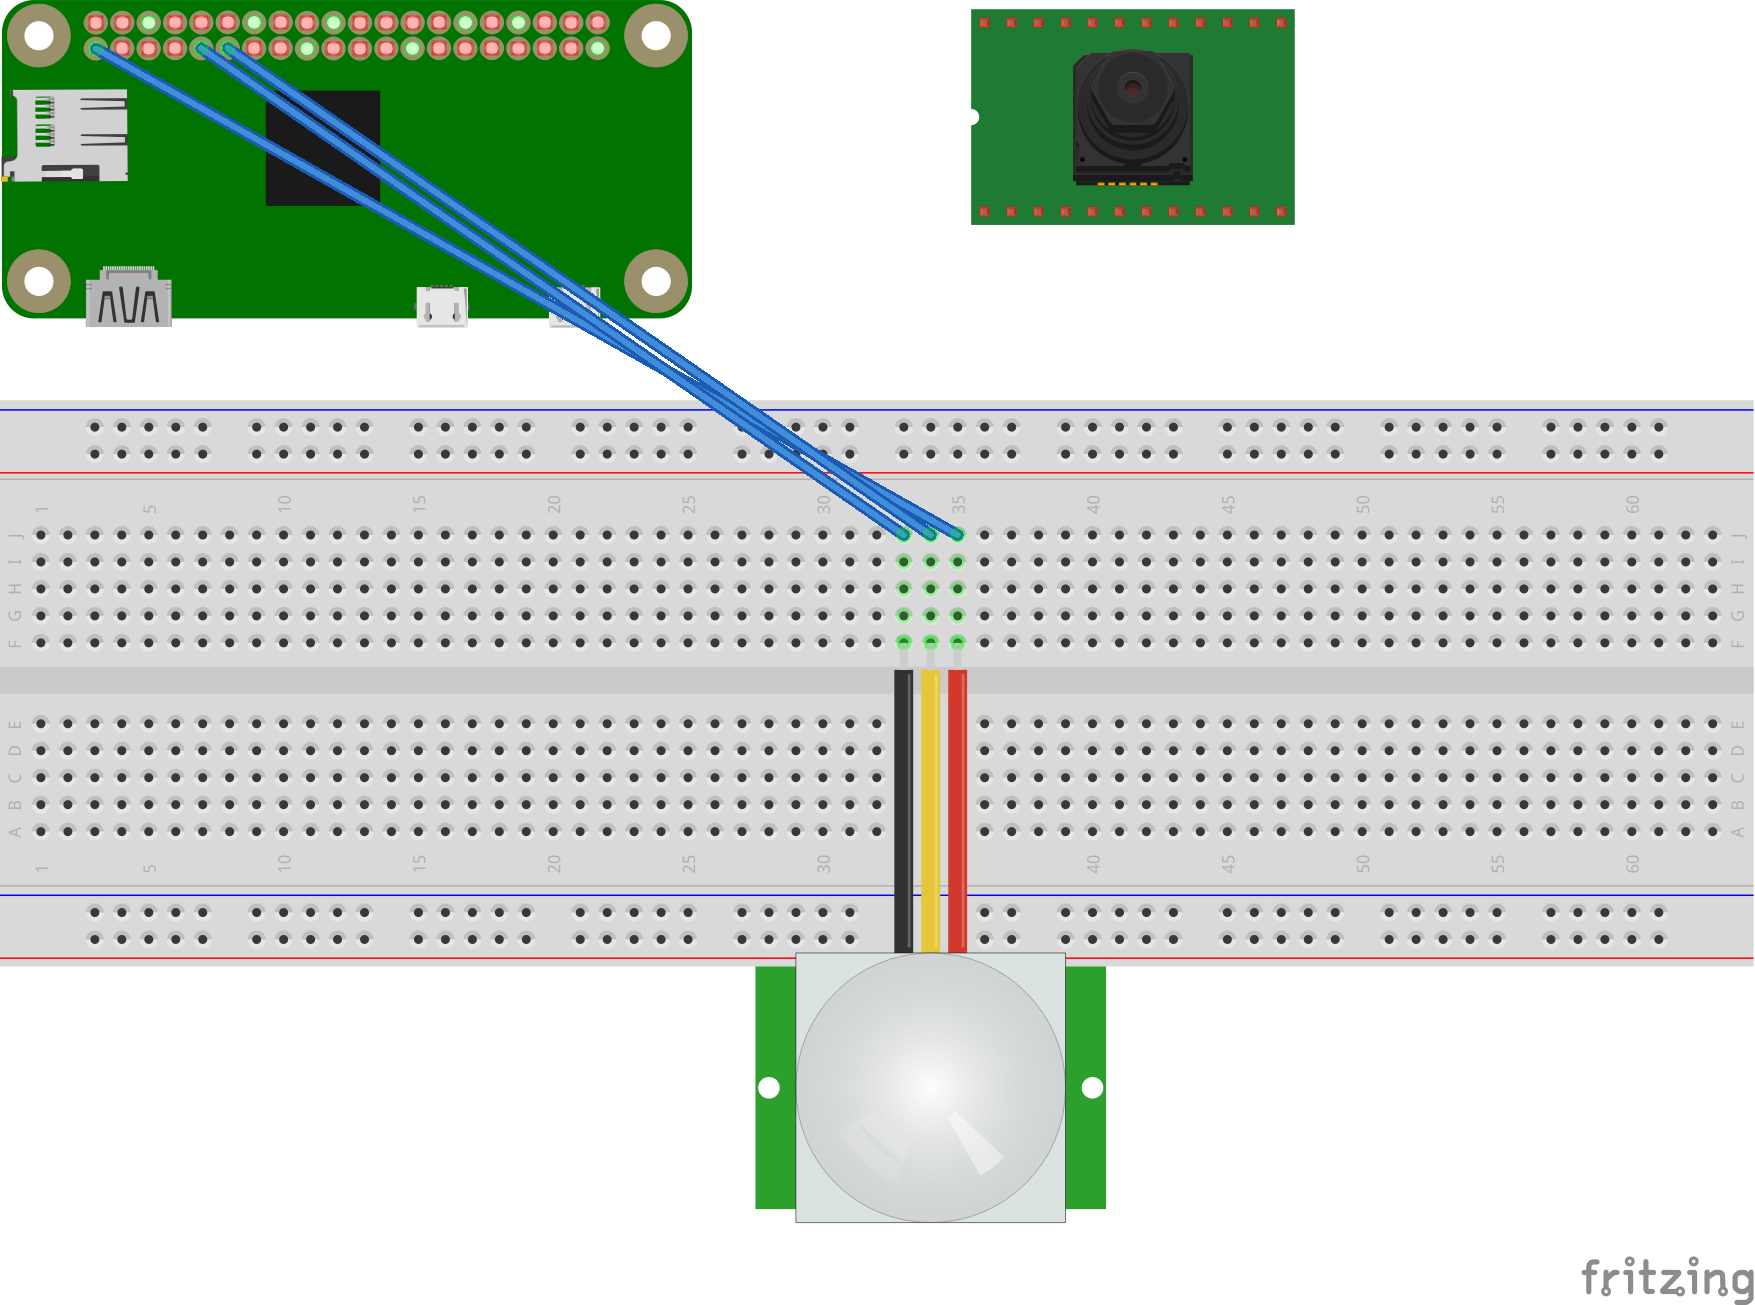
\includegraphics[width=\textwidth]{images/Schaltplan}
  \caption{Der Schaltplan}
\end{figure}